	\documentclass[../pfc.tex]{subfiles}
	
	\begin{document}
	
	El concepto de aplicación es un asistente-diario para un enfermo de cáncer en la parte de la app móvil y una parte servidora que se encarga de sincronizar datos entre diferentes dispositivo, una base datos para dar apoyo a esto y que ademas reciba datos estadísticos de la app, por si alguna vez pueden extraer conclusiones tras un tratamiento estadístico de los mismos. Además se incluye un servicio de comunicación con los usuarios mediante notificaciones push a los dispositivos\\*
	
	
	\section{Estado del arte de la movilidad}
	Dentro del concepto Movilidad se agrupan, tanto el hardware como el software de pequeños dispositivos portables o dispositivos móviles. Podríamos definir a estos últimos como “aparatos de pequeño tamaño, con algunas capacidades de procesamiento, con conexión permanente o intermitente a una red, con memoria limitada, diseñados específicamente para una función, pero que pueden llevar a cabo otras funciones más generales.”\\*
	
	De entre los elementos que pueden llegar a ser un dispositivo móvil (una PDA, un teléfono móvil, un lector de libros electrónico o un ordenador portátil) destaca, sin lugar a dudas, el teléfono móvil como el dispositivo más utilizado de entre todos. Y entre los teléfonos móviles destacan los denominados "SmartPhones y Tablets" por ser tener unas capacidades y potencia de ejecución de aplicaciones complejas de consumo de lo más variadas, desde reproductores de todo tipo de media, hasta mensajería instantáneas, llamadas apps. Es el desarrollo de estas apps y su comercialización por parte de grandes compañías tecnológicas como Google, Apple y Microsoft lo que ha devenido en todo un nuevo mercado de de desarrollo de software de todo tipo, no solo para grandes compañías sino también para pequeños grupos de desarrollo o incluso de desarrolladores indies. \\*
	
	\subsection{Smartphones}
	
	Un Smartphone (cuya traducción sería “teléfono inteligente”) “es una evolución del teléfono móvil tradicional que cuenta con ciertas características y prestaciones que lo acercan más a un ordenador personal que a un teléfono tradicional.”
	Entre dichas prestaciones y características, se encuentran una amplia mejora del almacenamiento de datos, conexión a Internet mediante una tarifa contratada o haciendo uso de redes WIFI, acelerómetro, pantalla táctil, teclado QWERTY ...y un sinfín de aplicaciones de usuario, además de la posibilidad de descarga de nuevas aplicaciones.\\
	Todas estas prestaciones y características de los Smartphone estarían desaprovechadas sin software que las saque partido. Por ello los Smartphone llevan un SO (Sistema Operativo) que les permite realizar todas estas tareas de una forma rápida y sencilla, además de optimizando el consumo energético ya que dependen de una batería para ello la mayoría de las veces. 
	En el siguiente apartado, realizaremos una breve descripción de los SO para dispositivos móviles y Smartphone más importantes que se encuentran en el mercado a día de hoy.\\*
	
	\subsection{Sistemas operativos Móviles}
	Partiendo de una definición de sistema operativo: “Capa compleja entre el hardware y el usuario, concebible también como una máquina virtual, que facilita al usuario o al programador las herramientas e interfaces adecuadas para realizar sus tareas informáticas, abstrayéndole de los complicados procesos necesarios para llevarlas a cabo.”\\*
	
	Por ende, un sistema operativo móvil es un sistema operativo que controla un dispositivo móvil. Sin embargo, estos son mucho muy diferentes a los tradicionales SO de equipos de escritorio, para empezar hay mucha mas variedad, pero es que la interacción con el usuario, la gestión de la memoria, las tareas de llamadas que deben ser prioritarias, etc\\*
	
	El sistema operativo destinado a controlar un dispositivo móvil necesita ser fiable y tener una gran estabilidad, ya que incidencias habituales y toleradas en ordenadores personales como reinicios o caídas no tienen cabida en un dispositivo de estas características. Además, ha de adaptarse adecuadamente a las consabidas limitaciones de memoria y procesamiento de datos, proporcionando una ejecución exacta y excepcionalmente rápida de cara al usuario.\\*
	
	Estos sistemas han de estar perfectamente testados y libres de errores antes de incorporarse definitivamente a la línea de producción. Las posibilidades que existen en un ordenador estándar de realizar actualizaciones e incluso reinstalar mejores versiones del sistema para cubrir fallos o deficiencias son más limitadas en un dispositivo móvil.\\*
	
	Es posible incluso que un aparato de esta naturaleza deba estar funcionando ininterrumpidamente durante semanas e incluso meses antes de ser apagado y reiniciado, a diferencia de lo que ocurre con un ordenador personal. El consumo de energía es otro tema muy delicado: es importante que el sistema operativo haga un uso lo más racional y provechoso posible de la batería, ya que esta es limitada y el usuario siempre exige una mayor autonomía.\\*
	
	En la actualidad, existen varios sistemas operativos para toda la gama de dispositivos móviles. Más adelante veremos por qué se ha elegido Android para la realización de este proyecto fin de carrera, pero antes veamos las características más importantes de los principales sistemas operativos móviles.\\*
	
	En 2015 en España y el mundo dentro de este mercado de SO de la movilidad se pueden encontrar diferentes actores que proveen de lo que denominamos sistemas operativos móviles, existiendo desde los provistos por las antes mencionadas grandes compañías tecnológicas hasta aquellos provistos por fundaciones, empresas que han perdido gran parte del negocio o empresas compradas por alguna de las grandes compañías, un repaso somero de los distintos SO móviles que podemos encontrar hoy día nos arroja nombres como Android, iOS, Windows Phone, Blackberry, Symbian, Firefox OS, Ubuntu Touch, etc\\*
		
	\section{¿Porqué Android?}
	
	Dentro del mercado de SO móviles solamente Android e iOS pueden considerarse grandes actores propiamente dichos pues entre ambos copan cerca del 90\% del mercado de Smartphones en España y más del 91\% mundial\cite{usomundso}. El resto algunas tuvieron gran peso pero hoy están en franca retirada (Blackberry), no terminan de funcionar todo lo bien que se desea entre el gran público (Windows Phone), son de dispositivos de "otra era" y no están pensados para la movilidad moderna (Symbian), o no terminan de salir del halo de prototipo y aun deben pasar ciclos en fases beta para  poder ser pasadas al gran público (Ubuntu Touch, Firefox OS).\\*
	
	\begin{figure}[h]
		\centering
		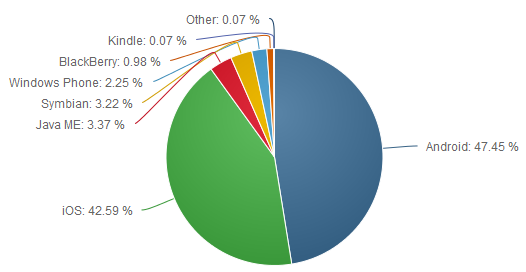
\includegraphics[width=0.8\linewidth]{../images/usomoviles}
		\caption{Gráfico sobre el uso actual de SO móviles internacional en Marzo de 2015.}
		\label{fig:usomoviles}
	\end{figure}
	
	Así pues la elección se encontraba entre Android e iOS de cara a afrontar este proyecto. Si tenemos en cuenta la cuota de mercado de cada uno de ellos, Android sin duda alguna es el gran vencedor, pero es que ademas la gama de dispositivos que ofrece dicho SO es bastante más amplia y con mayor variabilidad en el precio de los terminales, permitiendo que más y más personas accediesen a la app. \\*
	
	A esto hay que añadir los costes de desarrollo, ya que para publicar aplicaciones en las tiendas de las mismas de los SO móviles se necesita de un proceso de registro como tal desarrollador en las tiendas, y este proceso no es gratuito. Para ser claros diremos que el coste en iOS es de 99 dólares anuales, además de disponer de un hardware especifico para realizar el desarrollo y compilación de la app. Mientras que en Android el coste de de 25 dólares en un pago único y el desarrollo y compilación puede llevarse a cabo con casi cualquier infraestructura de SO, hardware etc. \\*
	
	Es por eso que para este piloto de la iniciativa de la Asociación Española contra el Cáncer se haya optado por un desarrollo más económico, y tras analizar los resultados si evalúa la iniciativa como positiva y avanza del estadio de piloto, se planteará por parte de la AECC futuros desarrollos en ese sentido, pero eso queda fuera del alcance y ámbito de este proyecto.\\*

	\section{Parte App móvil}
	
	En la parte de la app móvil hay 5 funcionalidades, aparte de los ajustes y preferencias, Personas Implicadas, Calendario de Citas y Posología, Seguimiento de Análisis, Rutina Diaria y Hablar con un agente, además de notificaciones locales preguntando por diferentes cosas, para mantener al usuario tanto en la app como con la moral lo más alta posible.\\*
	
	\textbf{Personas Implicadas} es una mini agenda personal, con el numero de teléfono o correo electrónico u otras formas de contacto de las personas que estén mas implicadas para el enfermo,se podrá especificar la relación que le une con el paciente, ya sea personal o derivada de su dolencia, como pueden ser su oncólogo, el agente de la AECC, un psicólogo propio, familiares o amigos de confianza con los que el agente de la AECC pueda contactar, previo consentimiento de estos y del paciente. En fin personas con interés en apoyar al enfermo en su duro trance de la enfermedad.\\*
	
	\textbf{Calendario de Citas y Posología} tiene como fin registrar las citas importantes relacionadas con el proceso del enfermo, como pueda ser revisiones, sesiones de quimio, entrega de análisis, ingresos, operaciones, etc Para que el enfermo disponga en un lugar de toda la información referente a su caso. Si toma algún medicamento, analgésico etc también se reflejar aquí como parte importante del proceso puramente médico en sí, esta parte constituye la funcionalidad principal y 'bebe' de la información y datos obtenidos de las otras secciones de la aplicación.\\*
	
	\textbf{Seguimiento de análisis} permite tener un pequeño histórico para el usuario de los análisis que le hayan sido realizados, permitiendo fotografiar los mismos para poder consultarlo siempre y ademas introducir que parámetros quiere obtener un especial seguimiento y gráfico de los mismos, es decir para ir comprobando su evolución \\*
	
	\textbf{Sintomatología} permite apuntar los síntomas que acontecen al paciente con fecha y hora de manera que estos puedan ser añadidos a la cita médica y sirvan de ayuda a la hora de hacer un diagnóstico más preciso de la situación de ese paciente, mejorando de manera directa su calidad de vida y el control de la enfermedad por parte de los facultativos al cargo del mismo.\\*
	
	\textbf{Rutina Diaria} tiene como finalidad la de ser un horario de actividades, tanto de dentro de la AECC como de fuera con la esperanza de que mediante la rutina y la realización de actividades el enfermo se encuentre mejor psicológicamente, además de físicamente en el caso de actividades físicas, y que mediante la rutina y realización activa de actividades consiga apartar de la mente la enfermedad, además el paciente podrá valorar de forma explícita el grado de satisfacción que le produce la realización de esta actividad.\\*
	
	\textbf{Hablar con un agente} permite durante ciertas horas del día que el enfermo pueda consultar o incluso simplemente charlar con el agente asignado de la AECC, para que sienta que siempre dispone de alguien que lo apoye desde el lado de la asociación.\\*
	  
	Ademas de esto la app dispone de preferencias tanto de sonidos y notificaciones como aspecto, así como ajustes de usuario borrar cuenta, etc\\*
	
	Por ultimo la app funcionará mucho en base a la información recolectada en esta parte para lanzar notificaciones locales preguntando por diferentes cosas al enfermo, desde como te encuentras esta mañana? a la hora aproximada que en Rutina Diaria el usuario haya establecido como hora de despertar a has ido hoy a bailes de salón? el día que tenga marcado que tiene que ir a bailes pasando que animo tienes? tras haber salido de una sesión de quimioterapia. Todos estos datos desagregados del usuario se envían a la parte servidora para tratarlos con fines estadísticos y ponerlos a disposición de investigadores en el campo de la enfermedad.\\*
	
	\section{Parte Servidora}
	
	La parte servidor lo primero que proporciona es una API REST(posible referencia) para interactuar con los recursos que ofrecerá.\\*
	
	Por una parte permite la sincronización de la información entre los diferentes dispositivos  que un mismo enfermo pueda disponer. Esto lo hace de manera silenciosa enviando cada cambio al servidor, y este en cada conexión de un dispositivo pregunta por su estado de sincronización.\\*
	
	Por otro ofrece servicios para que cada dispositivo envíe la información estadística pertinente, ademas la almacenará en una base de datos, haciendo anónimos esos datos en el proceso por confidencialidad hacia el usuario, y permitiendo después su consulta mediante servicio web o en la web donde este alojada la parte servidora, para la monitorización de los mismos.\\*
	
	Dispondrá de control de usuarios, esto es que existirá un usuario encargado de ir asignando a los distintos agentes, generalmente por proximidad geográfica, para que este sea el encargado de monitorizar la actividad de sus enfermos \\*
	
	Se le ofrecerá al agente los contactos de cada enfermo que tenga asignado para en el caso de que necesitase conversare de alguna manera con alguno de ellos, bien sean familiares o el oncólogo si por ejemplo se encuentra en algún ensayo poder contrastar información\\*
	
	En relación a esto ultimo la parte servidora dispondrá de un chat que permita comunicar directamente al agente con el enfermo, bajo ciertas premisas.\\* 
	
	\clearpage
	
	\section{Generación de la Documentación}
	
	Para la realización de la memoria, hemos elegido LaTeX y el editor TexStudio.
	
	LaTeX es un sistema de composición de textos de alta calidad; que incluye características diseñadas para la producción de documentación técnica y científica.
	
	LaTeX es el estándar de facto para la comunicación y publicación de documentos científicos y está disponible como software libre.\\*
	
	TexStudio es un entorno de escritura integrado para la creación de documentos LaTeX. 
	
	TexStudio hace la escritura LaTeX fácil y cómoda, tiene numerosas características como el resaltado de sintaxis, visor integrado, verificación de referencias y varios asistentes que hacen que introducir imágenes , tablas y diagramas sea sencillo. 
	
	TexStudio es de código abierto y está disponible para los principales sistemas operativos.
	
	\begin{figure}[H]
		\centering
		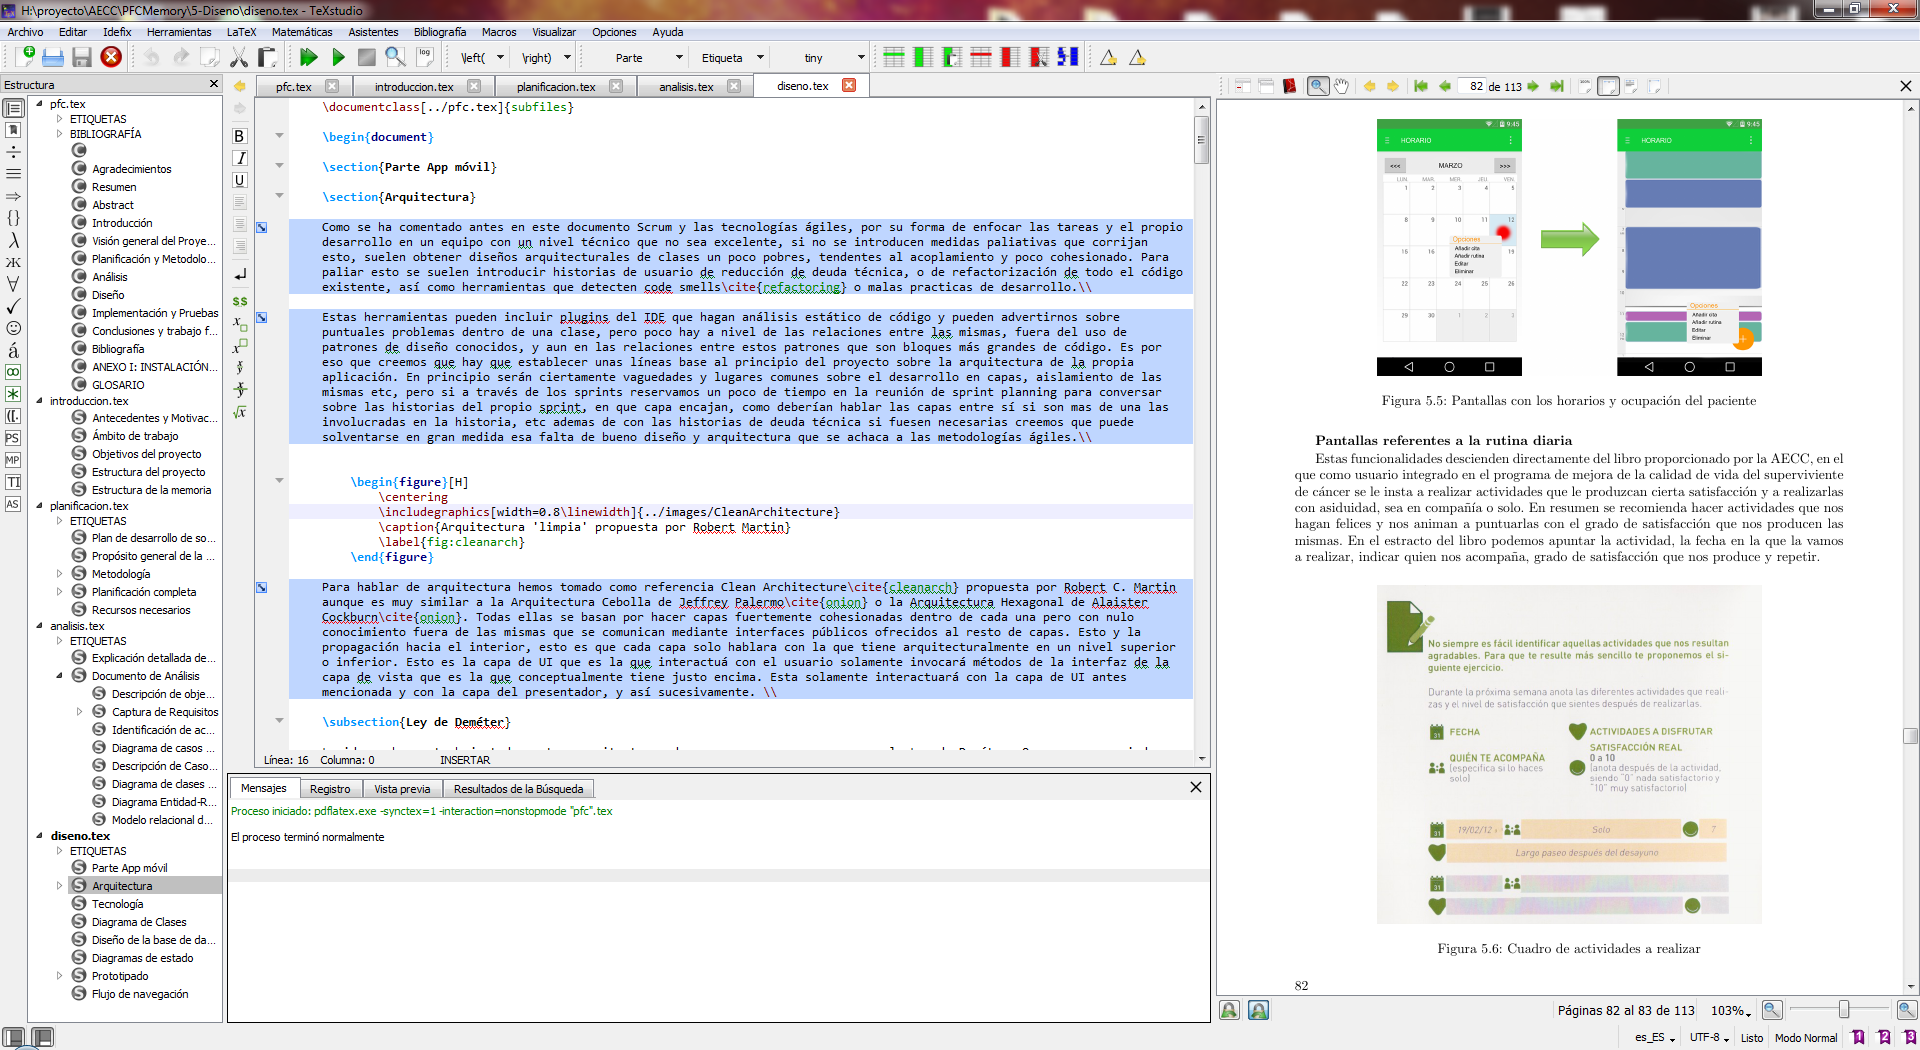
\includegraphics[width=1\linewidth]{../images/texstructura}
		\caption{Vista general de TexStudio}
		\label{fig:texstudio}
	\end{figure}
	
	TexStudio y LaTeX en general requieren de un aprendizaje, no es tan inmediata la generación de documentos con los formatos deseados como podría serlo Word, o incluso editores de texto online, del estilo a googleDocs, sin embargo, una vez que tienes el documento creado con las características deseadas, no es tan difícil de operar.\\*
	
	\clearpage

	TexStudio, utiliza por debajo de todo esto miktex que es una aplicación que se encarga de mantener actualizados todos estos paquetes a la última version y proporciona las funcionalidades que permiten que TexStudio genere los documentos.
	
	Aquí podemos ver la configuración del documento, paquetes necesarios, margenes, librerías de idioma,...
	


	\begin{figure}[H]
		\centering
		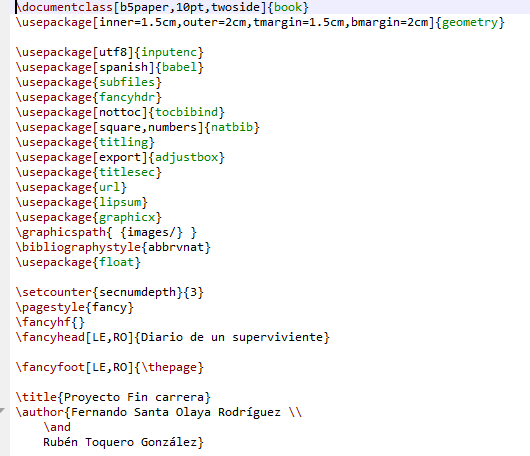
\includegraphics[width=0.7\linewidth]{../images/texstudiopack}
		\caption{Configuración del documento}
		\label{fig:texstudioPaQ}
	\end{figure}
	
	Una de las ventajas que nos han proporcionado LaTeX y TexStudio sobre el resto de los procesadores de texto ha sido el poder añadir sus archivos al repositorio, y poder tratar estos archivos de la misma manera que trataríamos cualquier archivo con una clase java o de otro tipo similar.\\*
	
	En principio el documento constaba de un .tex donde se realizaban todos los cambios para la generación del documento, sin embargo a medida que surgían los conflictos entre las versiones que subíamos al repositorio Git, decidimos particionar el .tex original en otros archivos del mismo tipo que fuesen llamados por el primero y que mantuviesen el formato y la configuración inicial.\\*
	
	Cada capítulo del libro pasó a ser un .tex independiente que se pudiese editar en TexStudio por separado y así minimizar los conflictos que iban surgiendo por la edición de la misma linea.\\*
	
	\begin{figure}[H]
		\centering
		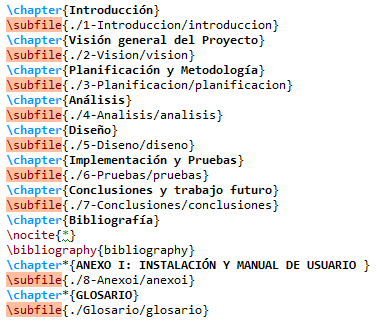
\includegraphics[width=0.5\linewidth]{../images/texstudiochapters}
		\caption{Capítulos dependientes del documento principal}
		\label{fig:texstudioCHAP}
	\end{figure}
	
	El documento inicial con las configuraciones y paquetes necesarios para la generación del documento junto a los capítulos del libro, Bibliografía y Glosario, forman el total del documento que es la memoria del proyecto.\\*
	
	

	
\end{document}